\documentclass[12pt]{article}
\usepackage{booktabs}
\usepackage{graphicx}
\usepackage{placeins}
\usepackage[left=2cm,right=2cm,top=2cm,bottom=2cm]{geometry}

\title{Exploiting Semantic Relationships for Word Sense Disambiguation}
\author{
       Tyler Folkman
            \and
	Sabarish Kumar
}
\date{May 15, 2015}

\begin{document}
\maketitle




\begin{abstract}


\end{abstract}




\section{Introduction}




\section{Problem Definition and Algorithm}


\subsection{Task Definition}


\subsection{Algorithm Definition}


\subsubsection{Lexical and Syntactic Features}


\subsubsection{Semantic Features}




\section{Experimental Evaluation}


\subsection{Methodology}


\subsection{Results}


\FloatBarrier
\begin{table}[h!]
\begin{tabular}{lrrrr}
\toprule
{} &  Random Forest &       SVM &  Ensemble 1 &  Ensemble 2 \\
\midrule
All Features       &       0.660851 &  0.704365 &    0.702876 &    0.696104 \\
Semantic Features  &       0.600540 &  0.634767 &    0.627087 &    0.621083 \\
Syntactic Features &       0.665298 &  0.699744 &    0.703718 &    0.698016 \\
\bottomrule
\end{tabular}
\caption{Average Results}
\end{table}
\FloatBarrier

\begin{figure}[h!]
\caption{Generous-a}
\centering
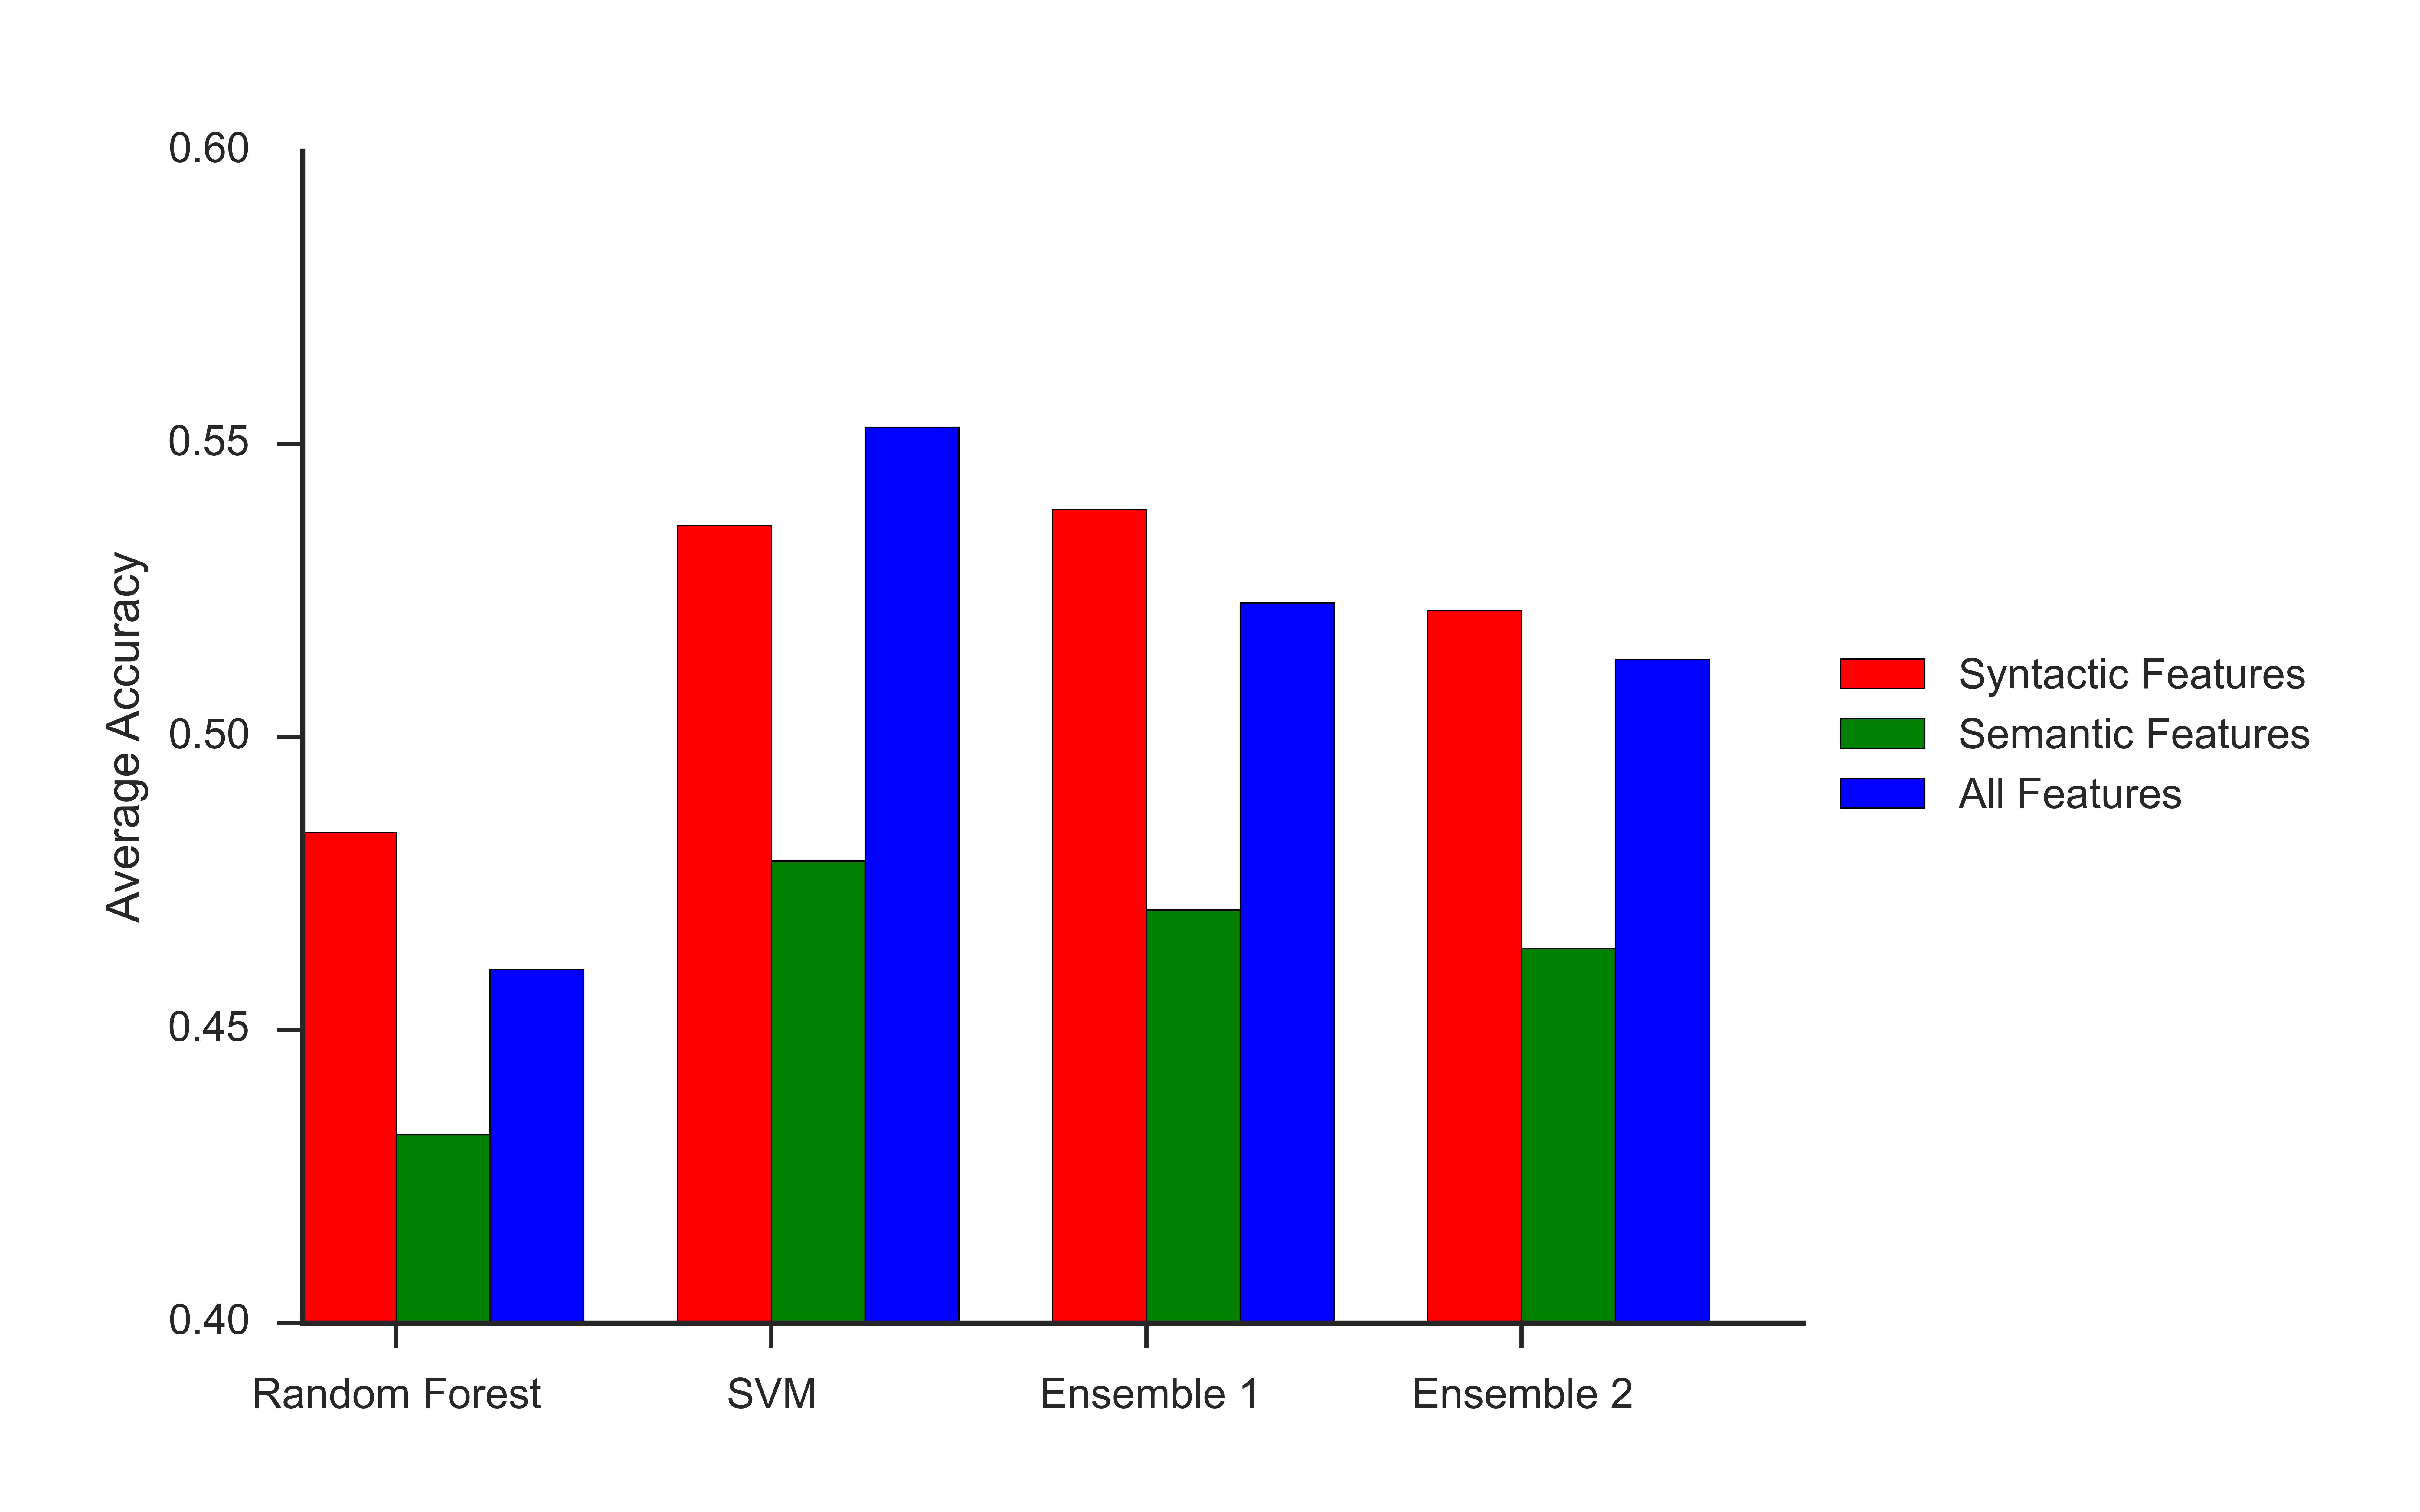
\includegraphics[width=1.0\textwidth]{../graphics/plots/generous-a.png}
\end{figure}
\FloatBarrier

\begin{figure}[h!]
\caption{Accident-n}
\centering
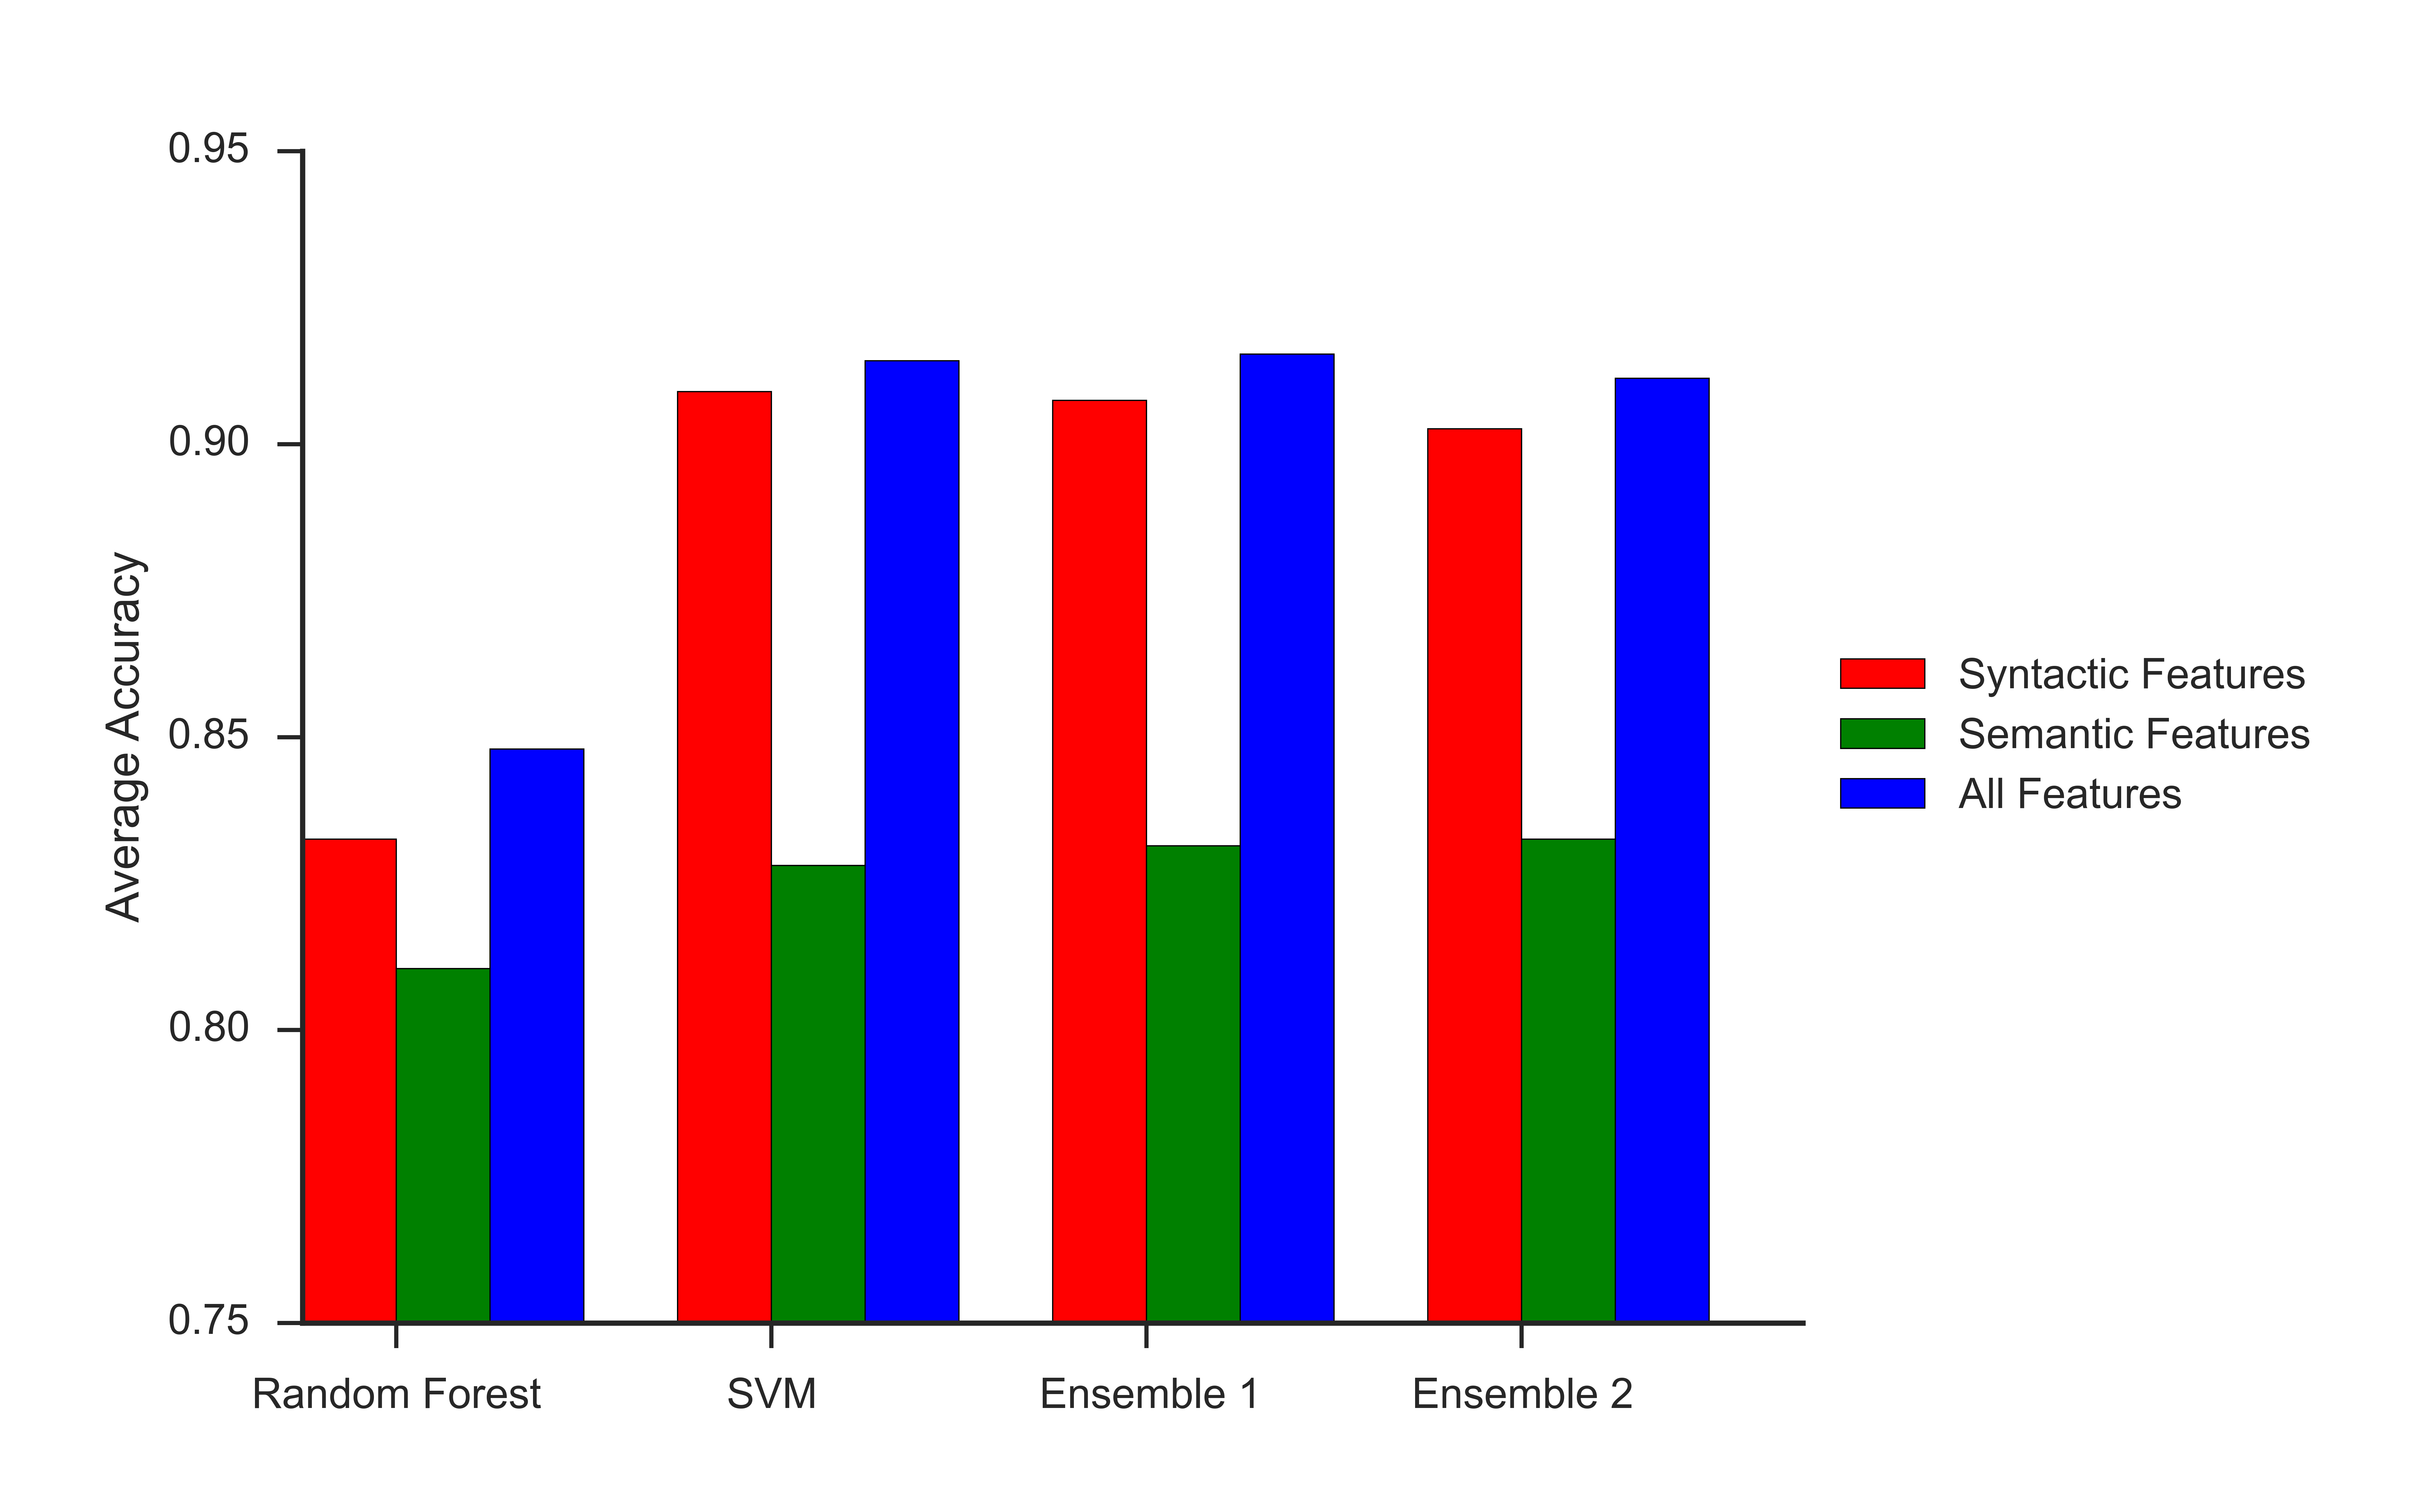
\includegraphics[width=1.0\textwidth]{../graphics/plots/accident-n.png}
\end{figure}
\FloatBarrier

\begin{figure}[h!]
\caption{Float-n}
\centering
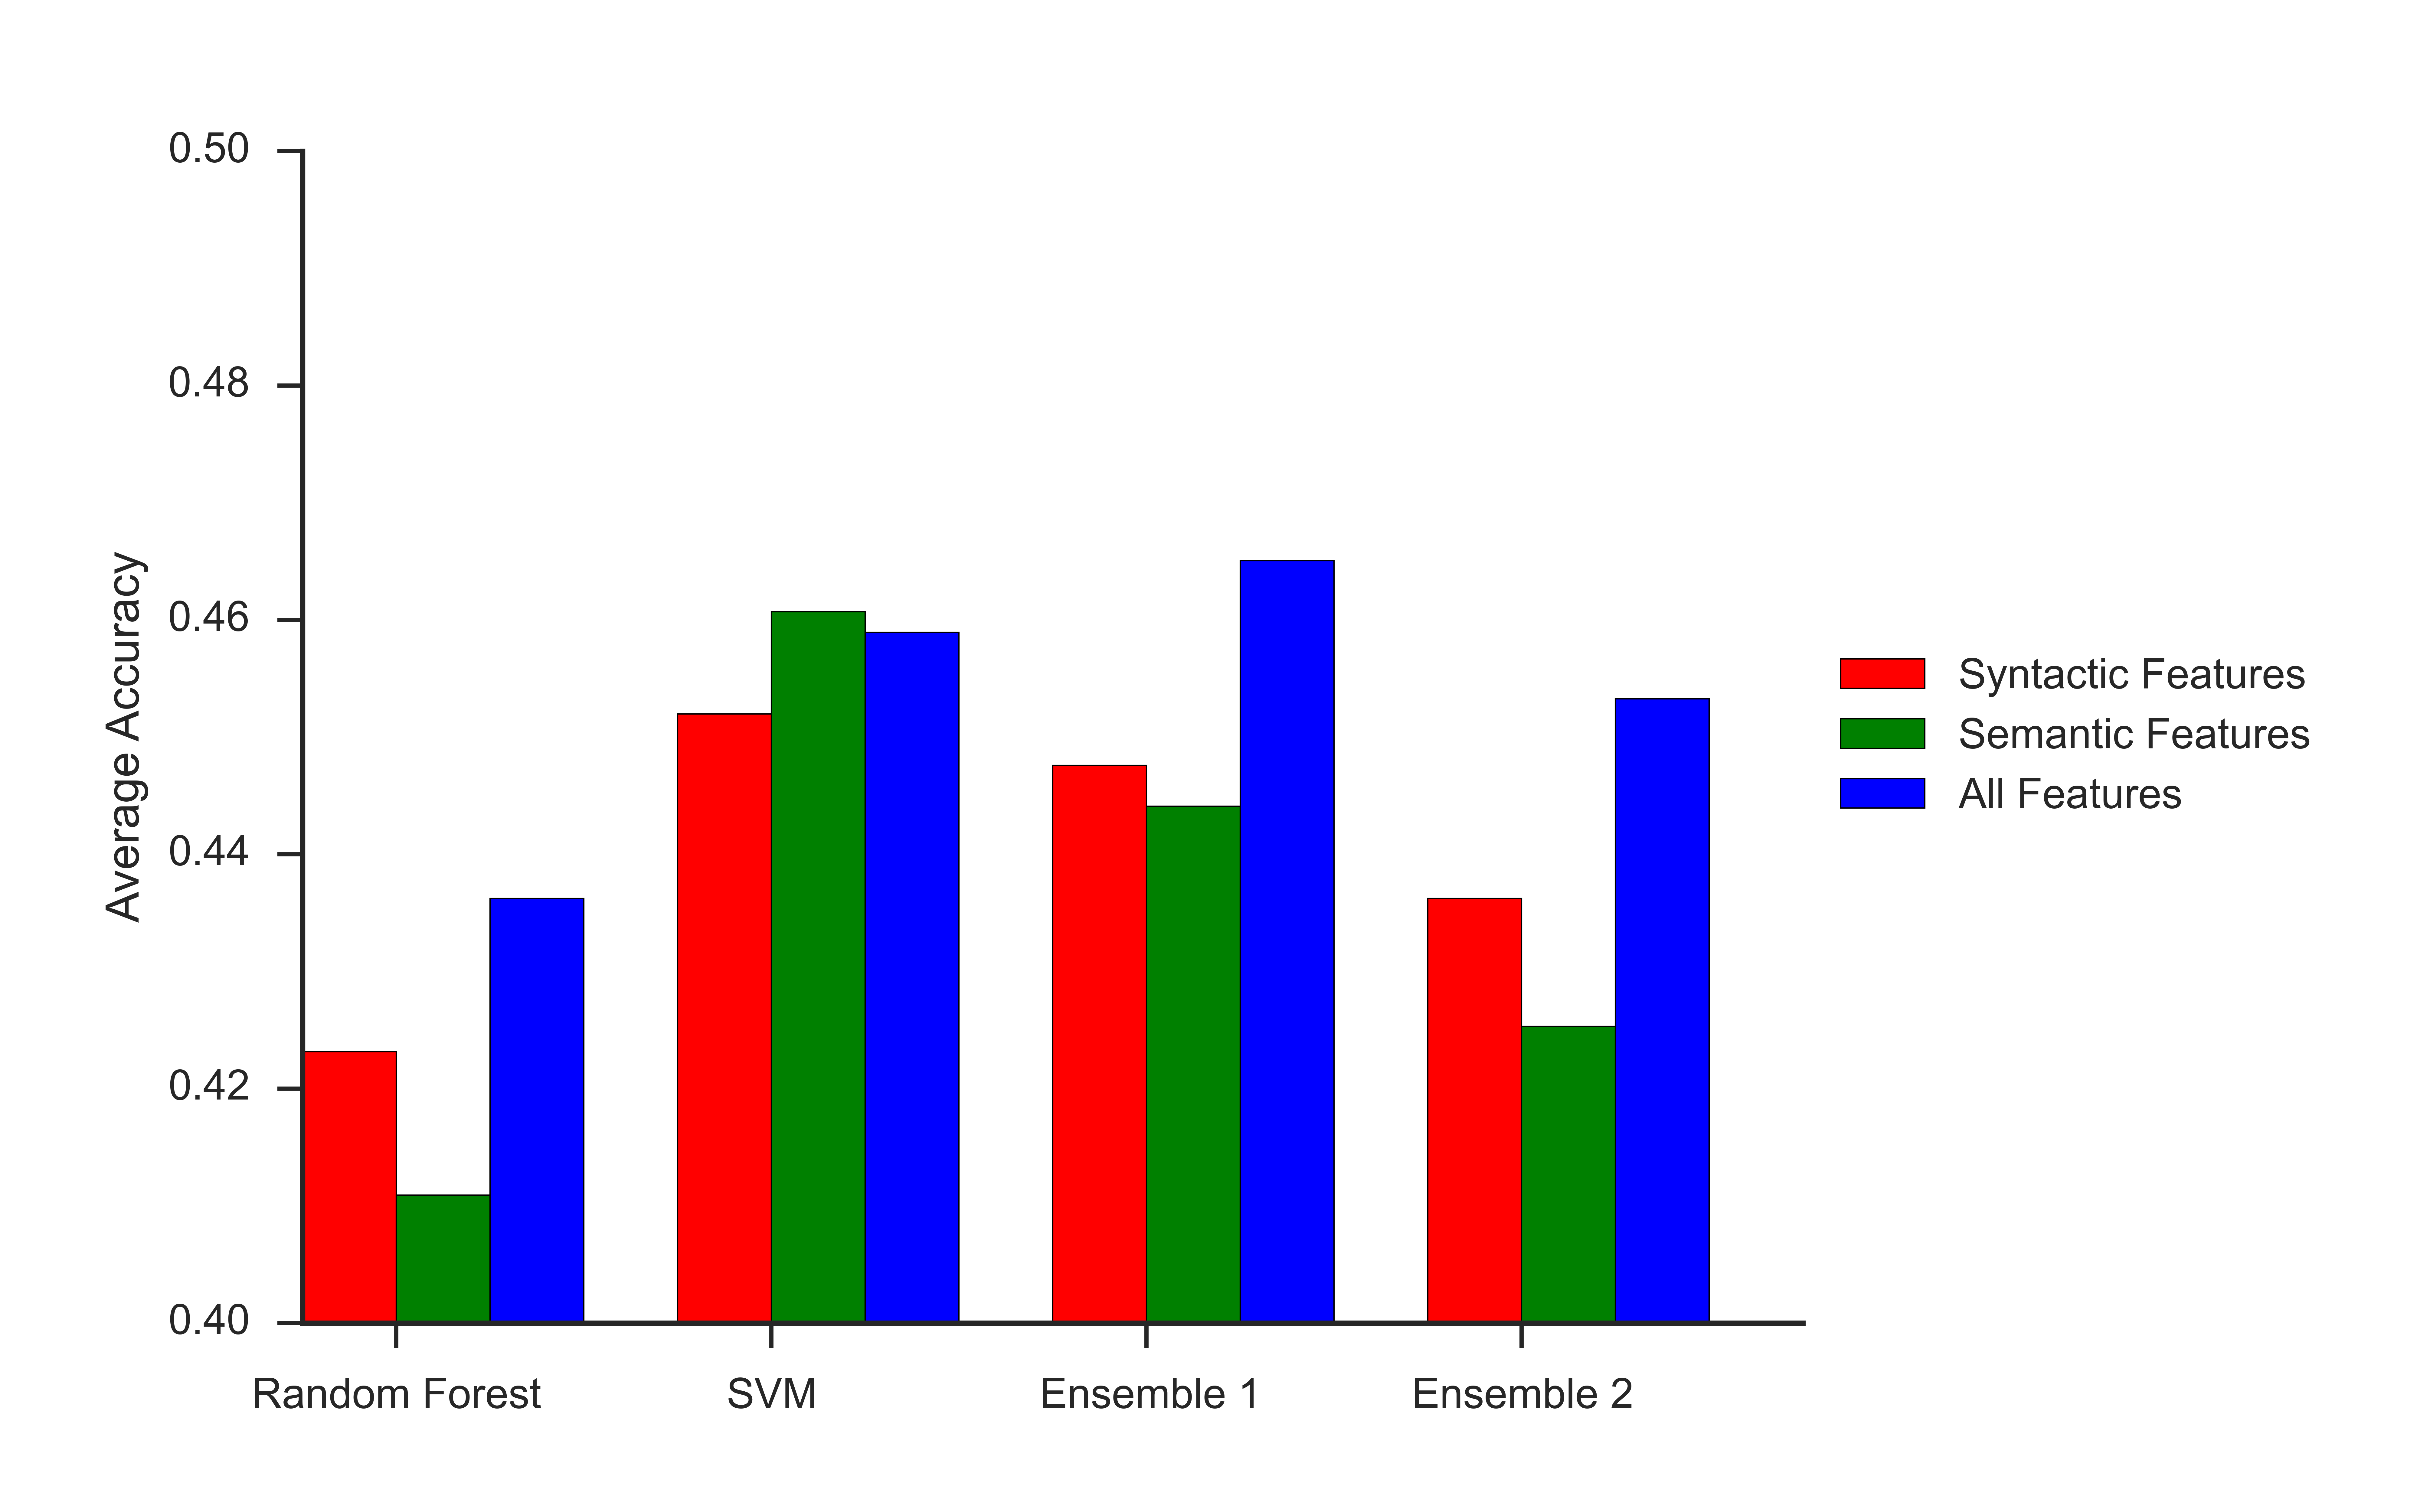
\includegraphics[width=1.0\textwidth]{../graphics/plots/float-v.png}
\end{figure}
\FloatBarrier


\subsection{Discussion}




\section{Related Work}




\section{Future Work}




\section{Conclusion}



\newpage
\section{Appendix}

\begin{tabular}{lrrrrl}
\toprule
{} &  Random Forest &       SVM &  Ensemble 1 &  Ensemble 2 &         Word \\
\midrule
All Features       &       0.847940 &  0.914232 &    0.915356 &    0.911236 &   accident-n \\
Semantic Features  &       0.810487 &  0.828090 &    0.831461 &    0.832584 &   accident-n \\
Syntactic Features &       0.832584 &  0.908989 &    0.907491 &    0.902622 &   accident-n \\
All Features       &       0.675120 &  0.727273 &    0.749282 &    0.740191 &     bother-v \\
Semantic Features  &       0.547368 &  0.583254 &    0.581340 &    0.575598 &     bother-v \\
Syntactic Features &       0.685167 &  0.740670 &    0.765550 &    0.759330 &     bother-v \\
All Features       &       0.482969 &  0.499563 &    0.490393 &    0.488646 &  brilliant-a \\
Semantic Features  &       0.472052 &  0.504367 &    0.489956 &    0.489956 &  brilliant-a \\
Syntactic Features &       0.473799 &  0.503930 &    0.482096 &    0.482096 &  brilliant-a \\
All Features       &       0.635023 &  0.658986 &    0.671429 &    0.671889 &     derive-v \\
Semantic Features  &       0.596774 &  0.623963 &    0.621659 &    0.616590 &     derive-v \\
Syntactic Features &       0.646083 &  0.627650 &    0.670046 &    0.663594 &     derive-v \\
All Features       &       0.773656 &  0.856452 &    0.824194 &    0.806989 &     excess-n \\
Semantic Features  &       0.636559 &  0.673118 &    0.660753 &    0.650000 &     excess-n \\
Syntactic Features &       0.787097 &  0.851613 &    0.829570 &    0.819892 &     excess-n \\
All Features       &       0.436245 &  0.458952 &    0.465066 &    0.453275 &      float-v \\
Semantic Features  &       0.410917 &  0.460699 &    0.444105 &    0.425328 &      float-v \\
Syntactic Features &       0.423144 &  0.451965 &    0.447598 &    0.436245 &      float-v \\
All Features       &       0.460352 &  0.552863 &    0.522907 &    0.513216 &   generous-a \\
Semantic Features  &       0.432159 &  0.478855 &    0.470485 &    0.463877 &   generous-a \\
Syntactic Features &       0.483700 &  0.536123 &    0.538767 &    0.521586 &   generous-a \\
All Features       &       0.865625 &  0.884375 &    0.884821 &    0.884375 &    promise-v \\
Semantic Features  &       0.847321 &  0.854464 &    0.851339 &    0.850446 &    promise-v \\
Syntactic Features &       0.868304 &  0.871875 &    0.882589 &    0.882143 &    promise-v \\
All Features       &       0.770732 &  0.786585 &    0.802439 &    0.795122 &       sack-n \\
Semantic Features  &       0.651220 &  0.706098 &    0.692683 &    0.685366 &       sack-n \\
Syntactic Features &       0.787805 &  0.804878 &    0.809756 &    0.814634 &       sack-n \\
\bottomrule
\end{tabular} 

\begin{thebibliography}{9}

\bibitem{se}
http://www.senseval.org/

\bibitem{kh}
K.L. Lee and H.T. Ng.  2002.  An empirical evaluation of knowledge sources and learning algorithms for word sense disambiguation.   In Proceedings of the Conference on Empirical Methods in Natural Language Processing, pages 41?48.

\bibitem{pend}
Pedersen, Ted, Mohammad, Saif  "Combining Lexical and Syntactic Features for Supervised Word Sense Disambiguation." Proceedings of the Conference on Computational Natural Language Learning (CoNLL), May 6-7, 2004, Boston, MA

\bibitem{amr}
"Abstract Meaning Representation for Sembanking" (L. Banarescu, C. Bonial, S. Cai, M. Georgescu, K. Griffitt, U. Hermjakob, K. Knight, P. Koehn, M. Palmer, N. Schneider), Proc. Linguistic Annotation Workshop, 2013. 

\bibitem{jamr}
JAMR - AMR Parser: https://github.com/jflanigan/jamr

\bibitem{syntalex}
Proceedings of the Third International Workshop on the Evaluation of Systems for the Semantic Analysis of Text (Senseval-3), pp. 159-162, July 25-26, 2004, Barcelona, Spain. 

\bibitem{sp}
Dan Klein and Christopher D. Manning. 2003. Accurate Unlexicalized Parsing. Proceedings of the 41st Meeting of the Association for Computational Linguistics, pp. 423-430. 

\bibitem{data}
http://www.d.umn.edu/~tpederse/data.html

\bibitem{recall}
Edmonds, Philip. "SENSEVAL: The evaluation of word sense disambiguation systems." ELRA newsletter 7.3 (2002): 5-14.

\end{thebibliography}

\end{document}






\begin{table}[h]
\begin{tabular}{l|lll}
\hline
Word      & Part of Speech & Training Size & Testing Size \\ \hline
Excess    & N              & 178           & 186          \\
Float     & V              & 183           & 229          \\
Brilliant & A              & 441           & 229          \\ 
Accident  & N              & 1,234         & 267          \\
Promise   & V              & 1,163         &   224          
\end{tabular}
\end{table}

\begin{table}[h]
\begin{tabular}{l|l}
\hline
Word      & Senseval Average  \\ \hline
Excess    & 0.652                     \\
Float     & 0.402                      \\
Brilliant & 0.443                      \\ 
Accident  & 0.802                   \\
Promise   & 0.741                      
\end{tabular}
\end{table}

\begin{verbatim}
(d / describe-01
    :arg0 (m / man)
    :arg1 (m2 / mission)
    :arg2 (d / disaster))
\end{verbatim}

\vspace{4mm}
The accident appeared to have little effect on the Christmas party, except to lengthen it considerably.
\vspace{4mm}

\noindent


  